%======================================================================
\documentclass[a4paper, 12pt]{article}
\usepackage[slovene]{babel}
\usepackage[utf8]{inputenc}

%oblika strani
\textwidth 15cm
\textheight 24cm
\oddsidemargin.5cm
\evensidemargin.5cm
\topmargin-5mm
\addtolength{\footskip}{10pt}
\pagestyle{plain}
\overfullrule=15pt

%slike
\usepackage{graphicx}
\graphicspath{{slike}}

%paketki
\usepackage{eurosym}

\usepackage{hyperref}
\hypersetup{
    colorlinks=true,
    linkcolor=black,
    filecolor=magenta,      
    urlcolor=cyan,
}

\urlstyle{same}


%slike
\usepackage{graphicx}
\graphicspath{{slike/}}
\usepackage{caption}
\usepackage{subcaption}

%======================================================================

\begin{document}

%======================================================================
%Naslovna stran
\thispagestyle{empty}
\noindent{\large
UNIVERZA V LJUBLJANI\\[1mm]
FAKULTETA ZA MATEMATIKO IN FIZIKO\\[5mm]
Finančna Matematika -- 1.~stopnja}
\vfill

\begin{center}{\large
Martin Kokošinek\\[2mm]
{\bf Analiza nogometnih transferjev FC Barcelona (2000-2020)}\\[10mm]
Projektna naloga pri predmetu Programiranje 1\\[1cm]
Predavatelj: prof. dr. Matija Pretnar}
\end{center}
\vfill

\noindent{\large
Ljubljana, 2020}
\pagebreak

%======================================================================
\thispagestyle{empty}
\tableofcontents
\pagebreak


\section{Uvod}
\begin{center}
{\bf Analiza nogometnih transferjev FC Barcelona (2000-2020)}\\[3mm]
{\sc Uvod} \\ \medskip
Pri predmetu programiranje 1 sem si za temo projektne naloge izbral analizo transferjev klub FC barcelona od sezone 2000/2001
do vključno sezone 2019/2020, brez poletnega prestopnega roka, saj v času pisanja, ta še ni bil zaključen.
Kot posameznik, ki v prostem rad spremljam dogajanje na nogometnih zelenicah klub FC Barcelona, me je, glede na dogajanje zadnjih let, zanimalo kako potekajo transferji kluba. 
V sezoni 2016/2017, ko se je zgodil senzacionalen prestop Neymarja iz FC Barcelona v PSG, za ogromnih \euro 222 mio., je cena prestopov na trgu igralec zelo zrasla. V luči tega dogodka, se mi je pojavilo nekaj vprašanj.\\

\begin{enumerate}
\item Kako je zrasla vrednost povprečenga nakupa po prodaji Neymarja (ali je zrasla?)
\item Število nakupov in prodaj (kako je bilo z nakupi v času 'zlate generacije' La Masie - manj?)
\item Ali Barcelona vedno več vlaga v nakupe in ali razlika med vrednostjo prihodov in odhodov raste?
\item So Brazilci v povprečju najdražji (pri prestopih) pri Barceloni?
\item Katere pozicije Barcelona največ 'kupuje' in katere 'prodaja'?
\end{enumerate}

Za odgovor na ta in podobna vprašanja, sem potreboval pridobiti podatke iz tabel na straneh Wikipedie na url linkih oblike \href{https://en.wikipedia.org/wiki/2000-01_FC_Barcelona_season#Transfers}{Transfer 2000-2001}. 
Za ta link in vse nadaljne sem moral pridobiti tabelo prestopov in jo nato urediti oziroma očistiti. Podatke, ki sem jih želel izluščiti so sledeči:
\begin{enumerate}
\item Ime
\item Državljanstvo
\item Vloga na igrišču (pozicija)
\item Klub iz katerega je prišel oziroma v katerega je šel igralec
\item Cena prestopa
\end{enumerate}

Tabele sem uvozil s pomočjo programskega jezika Python, knjižnice BeautifulSoup in priročnih orodij, ki nam jih je, za lažje delo, napisal profesor. 
Po urejanju tabel sem jih shranil v .csv datoteke in se lotil analize s pomočjo odprtokodne aplikacije Jupyter Notebook, kjer sem s knjižnico Pandas analiziral pridobljene podatke.

\end{center}
\pagebreak
%======================================================================
\section{Uvoz podatkov}

Projektna naloga je napisana v programskem jeziku python, kjer je glavni program za uvoz podatkov \textbf{Poberi\_podatke.py}.
Na začetku moramo shraniti html strani v neko mapo, da za vsako poizvedbo ne kličemo spletne strani ponovno. To izvedemo s pomočjo funkcije $shrani\_spletno\_stran$, ki je definirana v datoteki \textbf{orodja.py}.
Sedaj je potrebno iz dobljenih html strani pridobiti tabele. Tabele so se glede na leto razlikovale, prav tako pa njihovo stevilo na strani, kar lahko vidimo na sliki \ref{fig:htmlGET}. Zato definiramo funkciji $table\_IN(i,soup)$ in $table\_OUT(i,soup)$, kjer bo \textbf{i} predstavljalo sezono (za 2000/2001 je $i=2000$) in \textbf{soup} spletna stran pripravljena za branje s knjižnico BeautifulSoup. \\

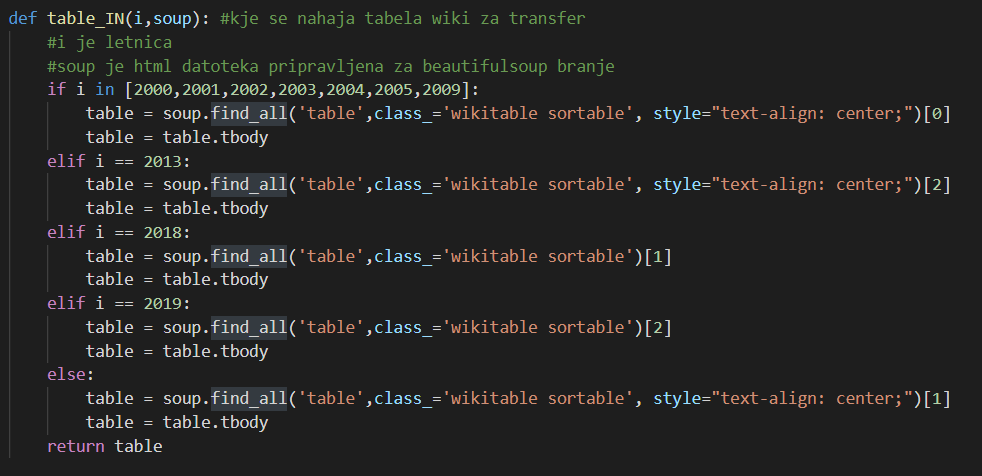
\includegraphics[width=0.9\textwidth]{html}
\captionof{figure}{Zgled funkcije $table\_IN$}
\label{fig:htmlGET}

Potem ko smo pridobili tabele, je bilo potrebno začeti iskati prave podatke, jih urediti in očistiti ter zapisati v tabelo primerno za shranjevanje v .csv datoteko.

\subsection{Čiščenje podatkov}
S pomočjo ukaza $\textbf{vrsticeIN}=tableIN.find\_all('tr')$, kjer \textbf{tableIN} predstavlja že pridobljeno tabelo, $find\_all('tr')$ pa poišče vse vrstice (table row) v tabeli. Nato s pomočjo ukaza $\textbf{dfIN} = pd.DataFrame(columns=stolpci)$ ustvarimo novo tabel (dataframe).
Tu nam $pd$ predstavlja okrajšavo za knjižnico Pandas, $columns=\textbf{stolpci}$ pa določi imena stolpcov, ki jih "pobere" iz seznama $\textbf{stolpci}$. Enako naredimo tudi za $\textbf{vrsticeOUT}$ in $\textbf{dfOUT}$. Primer IN lahko vidimo na sliki \ref{fig:htmlVrstice}.
\pagebreak

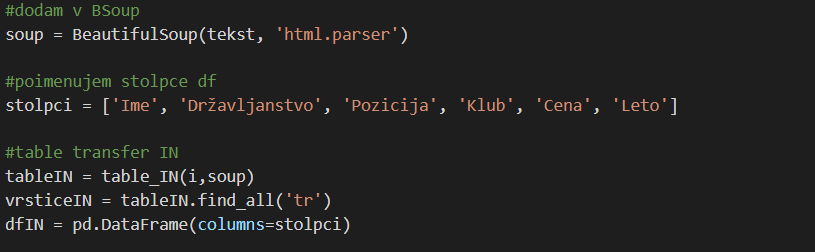
\includegraphics[width=\textwidth]{html2}
\captionof{figure}{Zgled priprave tabele}
\label{fig:htmlVrstice}

\subsection{Primer izluščevanja, čiščenja in shranjevanja podatkov}
Sedaj lahko zaženemo funkcijo $ustvari\_df(\textbf{vrsticeIN},\textbf{dfIN},\textbf{i},\textbf{\_})$, kjer $\_$ zavzame vrednost $'IN'$ ali $'OUT'$. V tej funkciji moramo za vsako vrednost \textbf{'tr'} poiskati vse vrednosti \textbf{'td'}. Zato izvedemo zanko $for$ na intervalu od 1 do dolžine $vrsticeIN$. Ker se tabele po letih razlikujejo (2018 in 2019 sta drugačni), je bilo potrebno ločiti tabele po letu 2017 in tabele do vključno leta 2017 in odvisno od smeri transferja prav tako. \medskip
\par V poročilu bom predstavil primer za sestavljanje tabel prihodov do leta 2017.\\
Za pridobivanje vrednosti v tabelah uporabimo $vrednost=[k.text for k in td]$, kjer $k.text$ vrne vrednost, ki je v tabeli in ne celotne vrstice td. Tu se nam pojavijo prvi problemi, za podatek o državljanstvu imamo na voljo ne ikono zastavice države iz katere je igralec. Država se nahaja pod tretjim stolpcem torej \textbf{td[3]}. 
Problem rešimo tako, da poiščemo kje v $<td>$ se nahaja ime države in odkrijemo, da se skriva pod \textbf{title}$=$ImeDržave. Nato z nekaj operacijami izluščimo ime države in ga shranimo v seznam \textbf{vrednost}, ki vsebuje podatke, ki jih zbiramo. \\
Za ostale podatke je dela manj, a vseeno gre omeniti vrednost prestopa, za katero je potrebno določiti nek skupen format izbral sem zapis v obliki miljonov in decimalno piko (brez valut, vedno gre za \euro). 
Naslednja posebnost, ki se je pojavila je bila neštevilčna vrednost prestopa (Free, Loan, Undisclosed, Youthsystem, \dots). Tu je potrebna obravnava za vsako posebnost posebej in izbrati najbol smiselno vrednost, ki ji pripada. V primeru Loan pa nogometaša odstranimo iz tabele, saj ta ne vpliva na ceno transferjev in ni dolgoročna okrepitev, torej analiza ni smiselna. Na slikah \ref{fig:htmlDrzava} in \ref{fig:htmlCSV} lahko vidimo kako smo izluščili državljanstvo in dobili ostale vrednosti ter kako smo ocistili vrednost prestopov, shranili oziroma dodali podatke v tabelo $dfIN$ in jih, po koncu izvajanja for zanke, zapisali v csv datoteko.

\pagebreak
\begin{center}
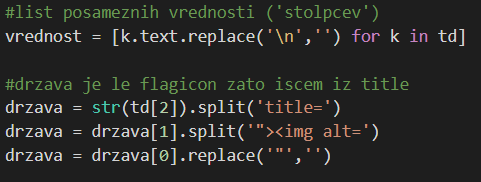
\includegraphics{html3}
\captionof{figure}{Izluščevanje državljanstva in pridobivanje vrednosti}
\label{fig:htmlDrzava}

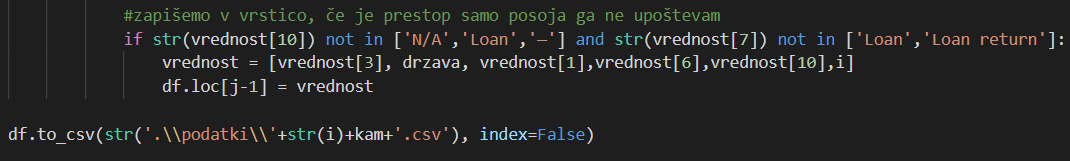
\includegraphics[width=1\textwidth]{html4}
\captionof{figure}{Čiščenje vrednosti prestopa in zapis v csv}
\label{fig:htmlCSV}
\end{center}
%======================================================================
\section{Analiza podatkov}
Sedaj, ko imamo podatke zbrane in očiščene ter shranjene v csv tabelah lahko začnemo z analizo. Najprej rabimo združiti tabele v skupni tabeli, eno za prihode in drugo za odhode kot je prikazano na sliki \ref{fig:analiza}. \\

\begin{center}
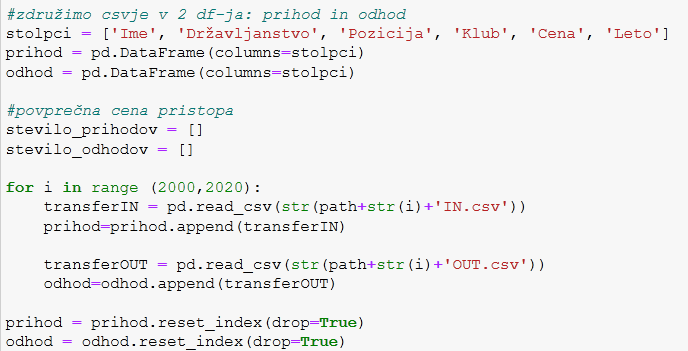
\includegraphics[width=0.9\textwidth]{analiza}
\captionof{figure}{Združevanje tabel v 2 skupni (prihod in odhod)}
\label{fig:analiza}
\end{center}

\subsection{Vpliv prestopa Neymarja na povprečno ceno}
Lotimo se prvega zastavljenega vprašanja torej ali in kako je zrasla povprečna cena prestopov po prestopu Neymarja. Po prestopu Neymarja je nogometni klub porabil več denarja kot ga je dobil od prestopa, prav tako pa lahko vidimo naraščajoč trend povprečnih cen prestopov, torej hipoteza drži. To lahko vidimo na sliki \ref{fig:graf1}, kjer črna navpična črta predstavlja prestop Neymarja.

\begin{center}
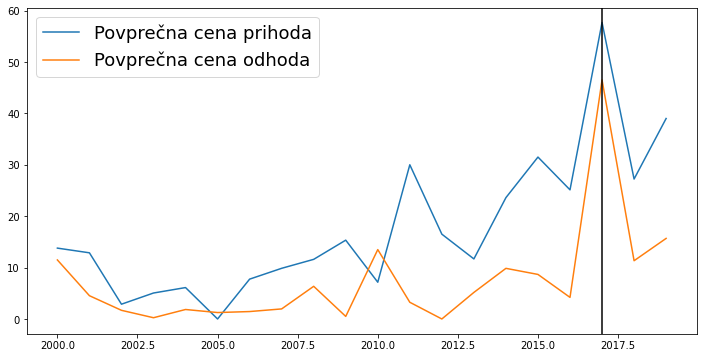
\includegraphics[width=0.9\textwidth]{graf1}
\captionof{figure}{Graf povprečnih cen prestopov}
\label{fig:graf1}
\end{center}

Za pridobitev tega podatka moramo najprej narediti poizvedbo po tabeli vseh prihodov imenovano \textbf{prihod}, jo združiti po letih $groupby('Leto')$ in izračunati povprečje $mean()$. Enako izvedemo na tabeli \textbf{odhod}. 
Za izris grafa pa uvozimo knjižnico $matplotlib.pyplot$ in z ukazom $plot()$ izrišemo graf. Primer je prikazan na sliki \ref{fig:analiza2}. Za nadaljne primere bomo le obrazložili kako smo prišli do željenih podatkov in ne kako poteka izris grafa.

\begin{center}
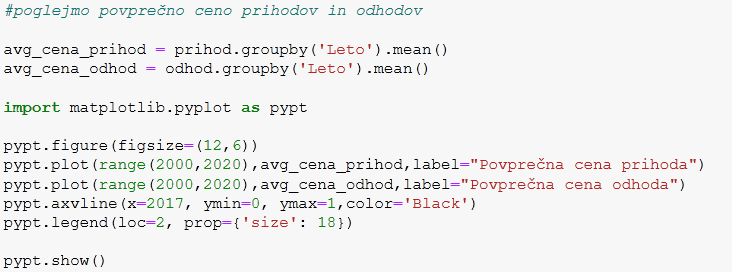
\includegraphics[width=0.9\textwidth]{analiza2}
\captionof{figure}{Izsek programske kode za izračun povprečnih vrednosti in izris grafa}
\label{fig:analiza2}
\end{center} \medskip

\subsection{Gibanje števila nakupov in prodaj}
Naslednje vprašanje, ki smo si ga zastavili je gibanje števila nakupov in prodaj s hipotezo kako je bilo z nakupi v času 'zlate generacije' La Masie jih je bilo manj. Za obdobje zlate generacije določimo obdobje od leta 2004 do leta 2012. Na sliki \ref{fig:graf2} lahko vidimo, da je graf prihodov v tem obdobju z izjemo leta 2010 pod grafom odhodov. Ta razlika pa je še bolj očitna na sliki \ref{fig:graf3}. Na obeh slikah je obdobje v rdečem pravokotniku.

\begin{minipage}{0.49\textwidth}
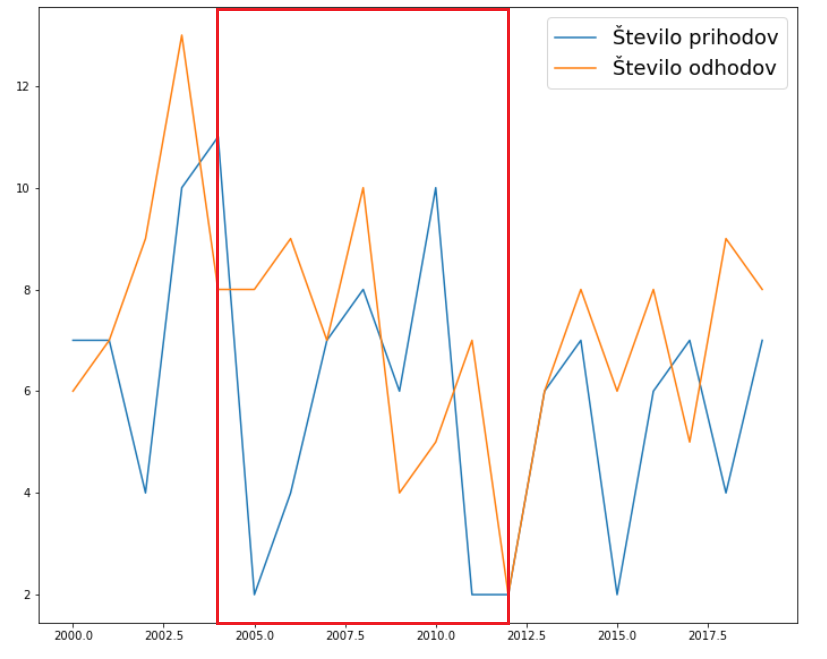
\includegraphics[width=1\textwidth]{graf2}
\captionof{figure}{Graf gibanja števila prihodov in odhodov}
\label{fig:graf2}
\end{minipage}
\begin{minipage}{0.49\textwidth}
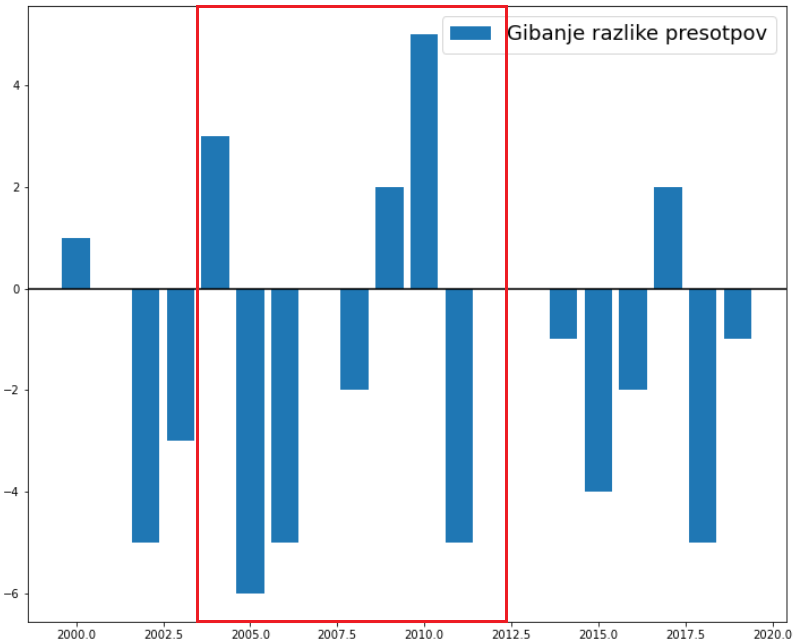
\includegraphics[width=1\textwidth]{graf3}
\captionof{figure}{Histogram gibanja razlike med prihodi in odhodi}
\label{fig:graf3}
\end{minipage} \medskip

Opazimo pa tudi, da ni bilo le obdobje zlate dobe La Masie tisto, ko je Barcelona več prodajala kot kupovala, ampak večinoma velja kar za celotno obdobje zadnjih 20 let. Torej hipoteza drži ampak, velja še več, saj je nakupov v splošnem manj kot prodaj.
Do teh podatkov smo prišli s pomočjo ukaza $prihod.groupby('Leto').size()$, ki nam na tabeli \textbf{prihod} združi prestope po letih, $size()$ pa vrne število vrstic, ki pripadajo posameznim letom. 
Razlika tega ukaza in analognega za odhod nam vrne gibanje števila razlike prihodov in odhodov, ki jo nato narišemo na graf. \medskip

\subsection{Cene prestopov}
Sedaj se nam pojavi tretje vprašanje. Torej kaj se dogaja s cenami prestopov in ali Barcelona v zadnjih dvajsetih letih služi s transferji. 
Za začetek si poglejmo razliko med vsoto odhodov po letih in vsoto prihodov po letih. Vsota vseh prihodov po letih lahko dobimo z ukazom $prihod.groupby('Leto').sum()$. Na sliki \ref{fig:graf4} vidimo kakšna je ta razlika po letih, na sliki \ref{fig:graf5} pa vidimo kako seštevek vložkov v prestope skozi leta raste, kjer so odhodi šteti negativno, prihodi pa pozitivno (da smo na pozitivnem delu osi y). Bolj natančne podatke pa na sliki \ref{fig:tabela1}.

\begin{center}
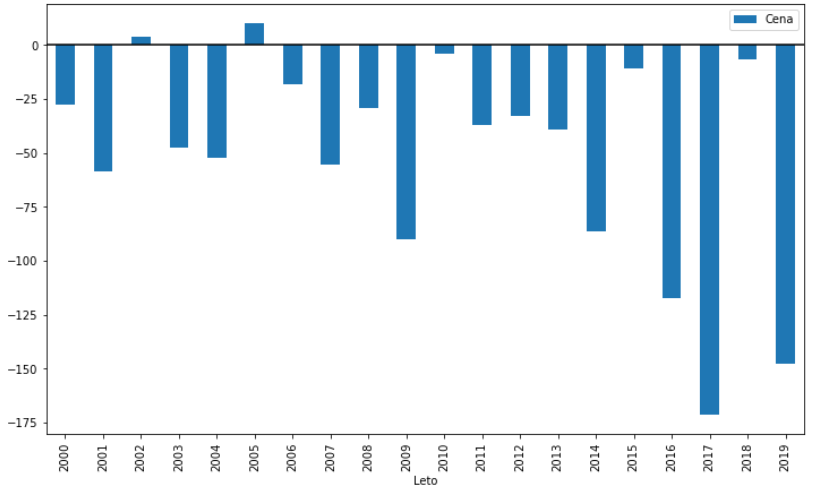
\includegraphics[width=0.7\textwidth]{graf4}
\captionof{figure}{Histogram gibanja razlike potrošnje za prestope}
\label{fig:graf4}

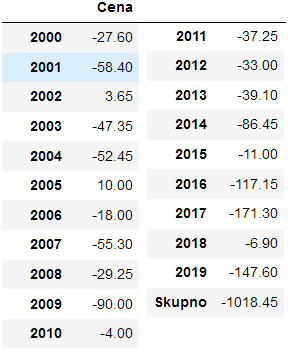
\includegraphics[width=0.45\textwidth]{tabela1}
\captionof{figure}{Histogram gibanja razlike potrošnje za prestope}
\label{fig:tabela1}

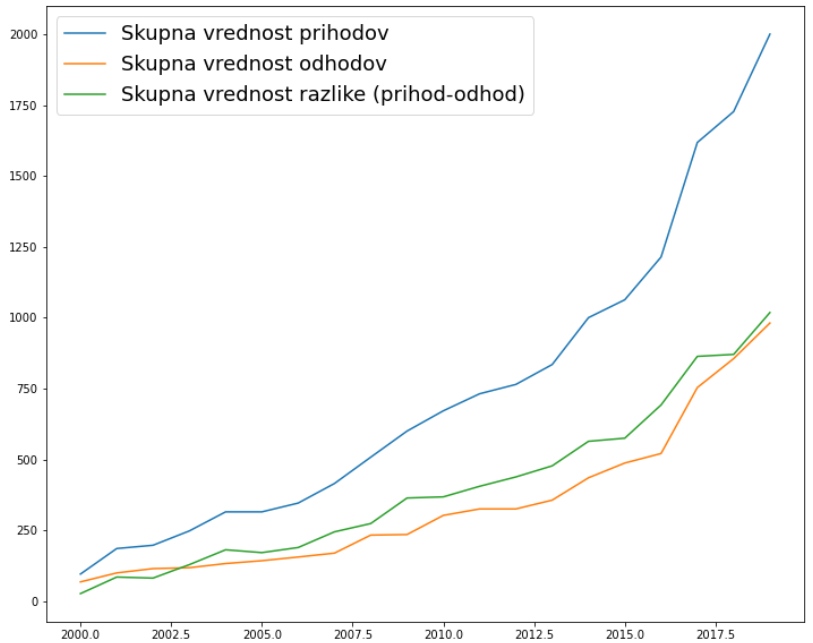
\includegraphics[width=0.75\textwidth]{graf5}
\captionof{figure}{Graf gibanja dohodkov, odhodkov in razlike transferjev}
\label{fig:graf5}
\end{center}

Izkaže se, da barcelona ne služi s transferji ampak ustvarja kar velik minus.
Zanimivo je opaziti vpliv prestopa Neymarja, ko je Barcelona v istem letu porabila skoraj še enkrat več kot je zanj dobila, da bi pokrila luknjo, ki jo je ustvaril njegov odhod.
Druga največja razlika se pojavi leta 2019. Verjetno najboljši igralec nogometa Lionel Messi se bliža koncu svoje kariere, zato je klub želel z njim osvojiti še čim več lovorik in posledično več vlagal v dražje nakupe oziroma igralce s takojšnim vplivom na igro (za razliko do vlaganje v mlade za prihodnost). 

\subsection{Razlika med skupno vrednostjo nakupov in skupno vrednostjo prodaj}
Barcelona ima dokaj strmo naraščanje razlike med skupno vrednostjo nakupov in skupno vrednostjo prodaj. Kar pomeni, da klub v splošnem skozi čas vedno več vlaga v nakupe, saj graf skupne vrednosti prodaj tudi raste. \\

Poglejmo s kakšno eksponentno funkcijo bi lahko v našem obdobju ocenili rast razlike ali tako imenovan postopek ``curve fitting''. Uporabimo knjižnico numpy in funkcijo $polyfit$. 
Ker imamo eksponentno funkcijo in rabimo polinom, ter so vse vrednosti razlike med skupno vrednostjo nakupov in skupno vrednostjo prodaj pozitivne, lahko brez težav logaritmiramo.
Naša funkcija bo oblike $y=e^{xb+a}$, torej bo polinom oblike $log(y)=xb+a$, to bodo podatki, ki jih bomo vstavili v funkcijo za iskanje najbolje prilegajoče funkcije po metodi najmanjših kvadratov. Zapis kode je na sliki \ref{fig:analiza3}. Funkcija $polyfit$ nam vrne koeficiente polinomov ter, če dodamo argument $full=True$ še druge podatke kot na primer vsoto kvadratov residualov (VKR), to je vsota kvadratov razlik med vrednostmi y in njihovimi ocenami (torej vsota kvadratov napak). 
Najbolje prilegajoča eksponentna funkcija je $e^{0.15x+4.26}$ z VKR=$1.37$. Graf prilegajoče funkcije je na sliki \ref{fig:graf7}.

\begin{center}
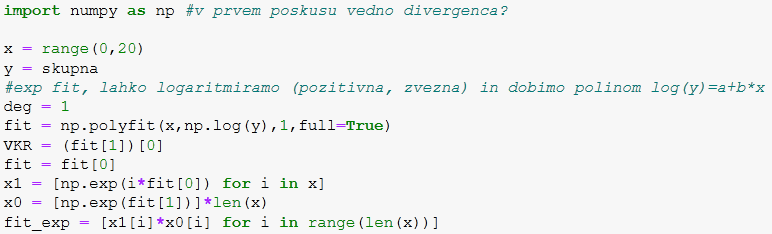
\includegraphics[width=0.9\textwidth]{analiza3}
\captionof{figure}{Koda s katero dobimo aproksimacijo naših podatkov z eksponentno funkcijo}
\label{fig:analiza3}

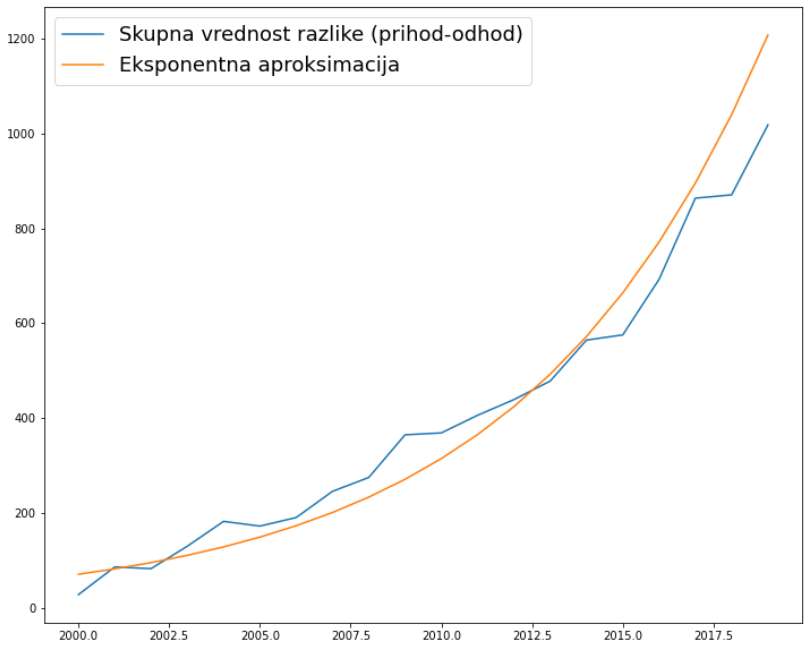
\includegraphics[width=0.7\textwidth]{graf7}
\captionof{figure}{Graf razlike med vrednostjo nakupov in skupno vrednostjo prodaj in njeno eksponentno aproksimacijo}
\label{fig:graf7}
\end{center}


\subsection{So Brazilci v povprečju najdražji?}
Sedaj nas zanima povprečna cena prestopa po državah, da vidimo katero državljanstvo imajo igralci, ki so najvec vpleteni v prestope. 
Ker gledamo povprečne vrednosti je treba paziti tudi koliko prestopov je bilo v opazovanem obdobju za posamezno državljanstvo. Zato si poglejmo vrednosti ko imamo vsaj 5 prestopov za državljanstvo in nato še za vsaj 10. Če bi izbrali brez omejitev so v povprečju najdražji prestopi igralci iz Rusije z vrednostjo v povprečju 40 milijonov \euro $\,$ ampak je ta prestop le en. Na slikah \ref{fig:tabela2} in \ref{fig:tabela3} je tabelarični prikaz povprečnih vrednosti prestopov po državljanstvih z vsaj 5 prestopi in vsaj 10 prestopi. Na sliki \ref{fig:tabela4} pa imamo vsote vseh prestopov, kjer vrednost preseže 50 milijonov \euro. 
\\
Opazimo, da v primeru, ko imamo vsaj 5 prestopov so v povprečju nadražji prestopi Portugalci s povprečno vrednostjo 26.28 milijona \euro. Za vrednosti nad 10 pa naša hipoteza drži saj so na najdražjem mestu Brazilci z vrednostjo 18.45 milijona \euro $\:$ in tudi na najdražjem mestu vsote vrednosti prestopov z vsoto 719.40 milijona \euro. Dokaj prepričljivo bi lahko rekli, da hipoteza drži.

\begin{minipage}[t]{0.3\textwidth}
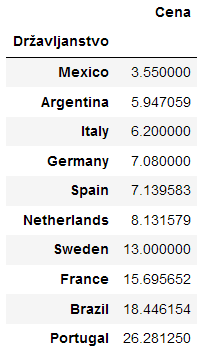
\includegraphics{tabela2}
\captionof{figure}{Povprečna vrednost prestopa (vsaj 5 prestopov)}
\label{fig:tabela2}
\end{minipage}
\hfill
\begin{minipage}[t]{0.3\textwidth}
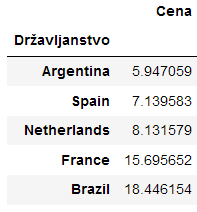
\includegraphics{tabela3}
\captionof{figure}{Povprečna vrednost prestopa (vsaj 10 prestopov)}
\label{fig:tabela3}
\end{minipage}
\hfill
\begin{minipage}[t]{0.3\textwidth}
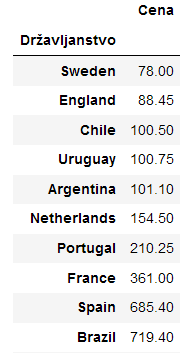
\includegraphics{tabela4}
\captionof{figure}{Skupna vrednost prestopov}
\label{fig:tabela4}
\end{minipage} 
\medskip

Željene podatke dobimo, tako da najprej združimo tabeli \textbf{prihod} in \textbf{odhod} v tabelo \textbf{vsi} z ukazom $prihod.append(odhod)$, ki doda tabeli \textbf{prihod} tabelo \textbf{odhod}. 
Nato razporedimo vse prestope prek ukaza $groupby.('Drzavljanstvo')$ jih seštejemo prek ukaza $sum()$, shranimo pod $x$ in izvedemo ukaz $[x>50].sort\_values('Cena').dropna()$. 
Ta ukaz nam vrne vse vsote nad 50 milijonov \euro $\:$, jih razporedi po ceni (padajoče) in zbriše vrednosti NaN. NaN bodo tiste vrednosti, kjer je vsota manjša od 50 milijonov \euro.

\subsubsection{Skupne cene prestopov po državah}
Dodatno lahko omenimo še, kako se gibajo skupne vrednosti prestopov za 4 države z največjo skupno vrednostjo, kar lahko vidimo na sliki \ref{fig:graf6}. Tu spet lahko opazimo vpliv prestopa Neymarja (Brazilija) in posledično nakupa Coutinha (Brazilija) v istem prestopnem roku in, ker je skupna vrednost teh dveh prestopov skoraj 400 mio. \euro, opazimo lahko velik skok skupne vrednosti za Brazilce.

\begin{center}
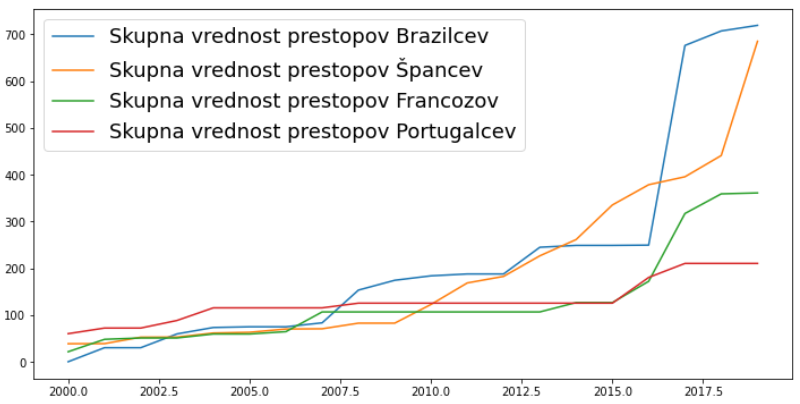
\includegraphics[width=0.9\textwidth]{graf6}
\captionof{figure}{Gibanje skupne vrednosti prestopov}
\label{fig:graf6} 
\end{center}

\subsection{Najbolje trgovane pozicije}
Za zaključek si odgovorimo še na zadnje vprašanje katere pozicije na igrišču so najbolj trgovane. Na slikah \ref{fig:tabela5}, \ref{fig:tabela6} in \ref{fig:tabela7} lahko po vrsti vidimo tabelo prihodov, odhodov in skupno. GK nam predstavlja vratarje, DF branilce, MF veziste in FW napadalce. Kar je tu pomembno opozoriti je, da pri skupni tabeli poizvedujemo po igralcih tako, da je prestop štet le enkrat tudi, če je igralec prestopil večkrat. To dosežemo z ukazom $vsi.drop\_duplicates(subset='Ime')$.\\


\begin{figure}[!htb]
\minipage{0.38\textwidth}
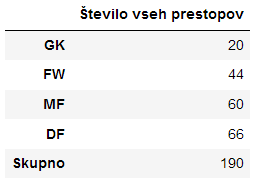
\includegraphics[width=\linewidth]{tabela5}
\caption{Število prestopov po pozicijah}\label{fig:tabela5}
\endminipage\hfill
\minipage{0.29\textwidth}
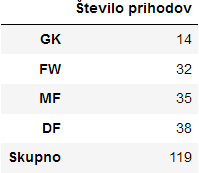
\includegraphics[width=\linewidth]{tabela6}
\caption{Število prihodov po pozicijah}\label{fig:tabela6}
\endminipage\hfill
\minipage{0.29\textwidth}
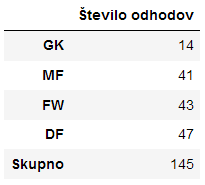
\includegraphics[width=\linewidth]{tabela7}
\caption{Število odhodov po pozicijah}\label{fig:tabela7}
\endminipage\hfill
\end{figure}

Tu je zanimivo opaziti, da je večina prihodov v Barcelono branilcev (DF), čeprav je nogometni klub taktično napadalno naravnan. Smiselna razlaga bi bila, da zaradi svoje filozofije ne "vzgojijo" $\:$ toliko branilcev in jih morajo posledično kupovati.



\pagebreak

\section{Zaključek}
S pomočjo uvoza podatkov in analize smo si uspeli odgovoriti na zastavljena vprašanja in sprejeli vse tri hipoteze. 

\begin{itemize}
\item Prestop Neymarja je imel vpliv na povprečno ceno prestopov, ta je višja kot pred letom 2017
\item Število nakupov v času zlate dobe La Masie je sicer res manjše od števila prodja, a to velja tudi v splošnem
\item Brazilci so res najdražji, če je prestopov določene države večje od 10, prav tako imajo največjo skupno vrednost
\end{itemize}

Pridobivanje podatkov je bilo močno olajšano s pomočjo knjižnice BeautifulSoup, saj ni bilo dela z regularnimi izrazi, kar bi zaradi raznolikosti tabel po letih, lahko pomenilo veliko dela z izluščevanjem tabel.\\
Večje število raznolikih podatkov nam omogoča več raznolike, natančnejše analize in lažje iskanje povezav med podatki oziroma vplivom dogodkov na podatke. Predvsem so zanimivi podatki gibanja skozi čas saj je pri njih aproksimiranje smiselno kot napoved prihodnosti. \\


%======================================================================
\end{document}